\documentclass[conference]{IEEEtran}
\IEEEoverridecommandlockouts
\usepackage{cite}
\usepackage{amsmath,amssymb,amsfonts}
\usepackage{algorithmic}
\usepackage{graphicx}
\usepackage{textcomp}
\usepackage{xcolor}
\usepackage{booktabs}
\usepackage{tikz}
\usepackage{url}
\usetikzlibrary{arrows.meta,positioning,shapes.geometric,fit,backgrounds}
\def\BibTeX{{\rm B\kern-.05em{\sc i\kern-.025em b}\kern-.08em
    T\kern-.1667em\lower.7ex\hbox{E}\kern-.125emX}}

\begin{document}

\title{Harness Engineering for LLM Agents: A Unified Reference Model,\\
Comparative Analysis of Self-Evolving Harnesses, and a Reporting Standard}

\author{
    \IEEEauthorblockN{First A. Author\textsuperscript{1}, Second B. Author\textsuperscript{1}, Third C. Author\textsuperscript{2}}
    \IEEEauthorblockA{
        \textsuperscript{1}Department of Computer Science, University Name, City, Country\\
        \textsuperscript{2}Department of Software Engineering, University Name, City, Country\\
        Email: \{first.author, second.author\}@univ.edu, third.author@univ.edu
    }
}

\maketitle

\begin{abstract}
An LLM agent is not a model alone: it is a model coupled to a \emph{harness}, the model-external runtime that constructs context, exposes tools, mediates actions, persists state, verifies results, and recovers from failure. With weights held fixed, changing only the harness moves task success by double-digit margins---for example, GPT-5 solves 35.2\% of Terminal-Bench 2.1 inside Terminus~2 but 49.6\% inside Codex CLI. Since the term ``harness engineering'' was named in early 2026, the field has produced at least four mutually incompatible taxonomies, four automated harness-evolution systems, and two large-scale empirical studies, yet no shared vocabulary or comparability protocol. This paper addresses that fragmentation. Our contributions are fourfold. First, we formalize the \emph{Unified Harness Reference Model} (UHRM), a canonical decomposition defined by sound projections and injectivity, and derive a 12-dimensional model that reconciles four independent taxonomies; the crosswalk exposes which concerns each taxonomy omits. Second, we define a ten-axis comparative protocol for self-evolving harness systems---adaptation locus, trigger, evidence, label access, selection rule, weight updates, persistence, transfer, failure modes, and safety reporting---and apply it to Agentic Harness Engineering, Self-Harness, TTHE, and HarnessDev. Third, we re-normalize every harness gain these systems report into a common effect scale, and show that the apparent ordering is an artifact of evaluation regime: test-time adaptation is transductive, creation studies use visible feedback, and slice-conditioned benchmarks inflate relative gains. Fourth, we propose the \emph{Harness Evolution Reporting Standard} (HERS), extending the Harness Condition Sheet with evolution-specific fields. Across all four systems, no governance or safety metric is reported for self-modified harnesses---a structural gap that we develop into a falsifiable research agenda.
\end{abstract}

\begin{IEEEkeywords}
harness engineering, LLM agents, coding agents, agent architecture, self-evolving agents, evaluation methodology, reproducibility, taxonomy
\end{IEEEkeywords}

\section{Introduction}

For most of the short history of large language model (LLM) agents, capability was attributed to the model. That attribution no longer holds for long-horizon work. An agent is a triple
\begin{equation}
\mathcal{A} = \langle M, H, E \rangle,
\end{equation}
where $M$ is the base model, $E$ the execution environment, and $H$ the \emph{harness}: the model-external runtime that determines which context is visible, which actions are available, where execution occurs, what state persists, how verification is performed, how failures are recovered, how work is delegated, and where governance is enforced~\cite{b7}.

The empirical case for treating $H$ as an object of study is now strong. HarnessDev reports that with \emph{identical} weights, GPT-5 solves 35.2\% of Terminal-Bench 2.1 inside one harness (Terminus~2) and 49.6\% inside another (Codex CLI)~\cite{b6}---a harness-induced swing of 14.4 percentage points, larger than the separation between many adjacent model generations. Self-Harness shows that editing only the harness raises pass rates on nine model--benchmark combinations, with a largest absolute gain of 40.6 points~\cite{b4}. Agentic Harness Engineering (AHE) lifts Terminal-Bench 2 pass@1 from 69.7\% to 77.0\%, surpassing a human-designed harness~\cite{b3}. Test-Time Harness Evolution (TTHE) improves a fixed ReAct~\cite{b9} baseline across five domains without any label access~\cite{b5}.

This activity has produced a vocabulary problem. The discipline was named in vendor engineering reports in early 2026~\cite{b19,b20} and given conceptual framings shortly afterwards, including a governance-oriented one~\cite{b8} and a concurrent source-level taxonomy of thirteen open-source scaffolds~\cite{b18}. At least four independent decompositions of the harness now coexist:
\begin{itemize}
    \item the \emph{seven canonical subsystems} of the Anatomy study~\cite{b1} (agent loop, LLM integration, tools, memory/context, safety, orchestration, extensibility);
    \item the \emph{ETCLOVG} seven-layer taxonomy of the Agent Harness Engineering survey~\cite{b2} (Execution, Tooling, Context, Lifecycle/Orchestration, Observability, Verification, Governance);
    \item the \emph{eight-function} Agent Harness Control Plane of~\cite{b7} (context ingress, action mediation, execution substrate, state persistence, verification, recovery, delegation, governance);
    \item the \emph{six-component} view reported by Meng et al.\ and adopted in~\cite{b2} (execution loop, tool registry, context manager, state store, lifecycle hooks, evaluation interface).
\end{itemize}
These decompositions are neither refinements nor coarsenings of one another. They disagree about whether observability and governance are first-class, whether recovery is distinct from verification, whether the execution substrate is part of the safety surface, and whether extensibility is a subsystem at all. Consequently, results reported under one decomposition are not directly interpretable under another, and the four automated evolution systems---AHE, Self-Harness, TTHE, and HarnessDev---each report gains under a different evaluation regime, a different notion of what is editable, and a different treatment of labels.

\subsection{Contributions}

This paper is a systematization and comparative analysis. It reports no new benchmark run; every quantitative claim is attributed to the source that published it, and every derived statistic is explicitly marked as our recomputation. We make four contributions.

\textbf{1) A unified reference model (Section~\ref{sec:uhrm}).} We formalize what it means for taxonomies of the harness to be \emph{compatible}, via sound projections and an injectivity requirement, and derive the coarsest canonical model satisfying them. The resulting 12-dimensional UHRM reconciles the four taxonomies above and yields a crosswalk (Table~\ref{tab:crosswalk}) that exposes, per taxonomy, which concerns it omits. Model/provider integration and extensibility are named by only one taxonomy each; recovery is first-class in only one; observability in only one.

\textbf{2) A comparative protocol for self-evolving harnesses (Section~\ref{sec:comparative}).} We define ten axes along which harness-adaptation systems must be described, and apply them to the four systems. The protocol makes explicit a property shared by all four---base weights are frozen---and a property on which they diverge completely: label access.

\textbf{3) A normalized synthesis of reported gains (Section~\ref{sec:synthesis}).} We re-express every reported harness gain on a common ceiling-normalized scale $\gamma$, and show that the resulting ordering is governed by evaluation regime rather than by method quality. We identify four confounds---transductive evaluation, visible feedback, slice conditioning, and ceiling effects---that the current literature does not control.

\textbf{4) A reporting standard (Section~\ref{sec:hers}).} We extend the Harness Condition Sheet of~\cite{b7} with evolution-specific fields to form the Harness Evolution Reporting Standard (HERS), and we note a uniform omission: none of the four self-evolution systems reports a safety or governance metric for its self-modified harness (Section~\ref{sec:open}).

\section{Background: From Prompt to Harness Engineering}
\label{sec:background}

\subsection{What a Harness Is, and Is Not}

We adopt the definition of~\cite{b7}: the harness is the model-external layer that determines which context is visible, which actions are available, where execution occurs, what state persists, how verification is performed, how failures are recovered, how work is delegated, and where governance is enforced. Two boundary cases matter for reading the literature. First, a harness is not an \emph{evaluation} harness: a SWE-bench harness wraps an agent to run it against tasks, whereas an agent harness wraps a model to make it act---the same word with the direction of wrapping reversed~\cite{b1}. Second, a harness is not an \emph{orchestrator} or \emph{meta-harness}: an orchestration layer such as Omnigent coordinates several harnesses from above but implements no editing loop of its own~\cite{b1}.

Fig.~\ref{fig:scope} situates harness engineering in the widening sequence from prompt engineering, to context engineering, to the surrounding execution system. The sequence is not a hierarchy of importance but an expanding engineering surface: each stage subsumes the artifacts of the previous one while adding new failure modes that cannot be addressed at the earlier stage.

\begin{figure}[t]
\centering
\resizebox{\columnwidth}{!}{%
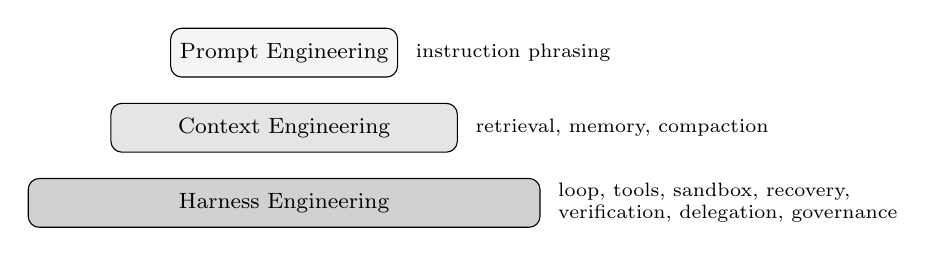
\begin{tikzpicture}[font=\footnotesize,node distance=3.2mm]
\node[draw,rounded corners,fill=black!4,minimum width=2.6cm,minimum height=0.62cm] (p) {Prompt Engineering};
\node[draw,rounded corners,fill=black!10,below=of p,minimum width=4.4cm,minimum height=0.62cm] (c) {Context Engineering};
\node[draw,rounded corners,fill=black!18,below=of c,minimum width=6.5cm,minimum height=0.62cm] (h) {Harness Engineering};
\node[font=\scriptsize,right=1mm of p,align=left] {instruction phrasing};
\node[font=\scriptsize,right=1mm of c,align=left] {retrieval, memory, compaction};
\node[font=\scriptsize,right=1mm of h,align=left] {loop, tools, sandbox, recovery,\\ verification, delegation, governance};
\end{tikzpicture}}

\caption{The widening engineering surface. Harness engineering subsumes prompt and context engineering while adding runtime concerns---execution substrate, recovery, delegation, and governance---that neither earlier stage can express.}
\label{fig:scope}
\end{figure}

\subsection{The Four Taxonomies}

Table~\ref{tab:taxonomies} lists the four decompositions and their dimensions. The Anatomy study derives its seven subsystems from source-level analysis of eleven production coding harnesses plus a meta-harness, across roughly four million lines of Python, TypeScript, and Rust~\cite{b1}. The ETCLOVG taxonomy is the product of a survey that codes more than 170 open-source projects against seven layers~\cite{b2}. The Control Plane decomposition is a conceptual framework validated against seven systems and four evidence classes~\cite{b7}. The six-component view is a component-level description of an individual harness~\cite{b2}.

The taxonomies were derived by different methods (source audit, ecosystem coding, conceptual formalization, component description), for different purposes (describing artifacts, mapping an ecosystem, analyzing control, specifying a single system), and at different granularities. Compatibility is therefore not automatic, which is precisely the problem Section~\ref{sec:uhrm} addresses.

\begin{table*}[t]
\caption{The four coexisting decompositions of the agent harness.}
\label{tab:taxonomies}
\centering
\footnotesize
\begin{tabular}{@{}p{2.6cm}p{4.3cm}p{4.5cm}p{4.6cm}@{}}
\toprule
\textbf{Source} & \textbf{Method} & \textbf{Scope} & \textbf{Dimensions} \\
\midrule
Anatomy et al.~\cite{b1} & Source-code audit of 12 systems ($\approx$4M LOC) & Artifact anatomy & Agent loop; LLM integration; tools \& actions; memory \& context; safety \& permissions; orchestration; extensibility \\
ETCLOVG~\cite{b2} & Coding protocol over 170+ projects & Ecosystem mapping & Execution env.; Tool interface; Context mgmt.; Lifecycle/Orchestration; Observability; Verification; Governance \\
Control Plane~\cite{b7} & Conceptual formalization, 7 systems, 4 evidence classes & Control analysis & Context ingress; action mediation; execution substrate; state persistence; verification/review; recovery/debugging; delegation/coordination; governance/audit \\
Component view~\cite{b2} & Component description of one harness & Single system & Execution loop; tool registry; context manager; state store; lifecycle hooks; evaluation interface \\
\bottomrule
\end{tabular}
\end{table*}

\subsection{Self-Evolving Harness Systems}

Four systems automate harness improvement while holding base weights fixed. They are not the first mechanisms to adapt an LLM system without touching weights: verbal self-reflection revises a single response or stores textual experience for later attempts~\cite{b16}, and declarative pipeline compilation searches over prompts and control flow~\cite{b17}. Both, however, treat the adaptation target as a response or a pipeline rather than as the runtime that mediates the agent's entire interaction with its environment. AHE~\cite{b3} exposes seven editable harness component types as files and drives a closed evolution loop through three ``observability pillars'' (component, experience, and decision observability), where each edit carries a self-declared prediction that is later verified against the next round's task-level outcomes. Self-Harness~\cite{b4} runs a three-stage loop---Weakness Mining over clustered execution traces, Harness Proposal of minimal edits tied to identified failures, and Proposal Validation by regression testing. TTHE~\cite{b5} moves adaptation into evaluation itself, maintaining a population of candidate harnesses, refining them with an agentic proposer over unlabeled execution traces, and committing one via a judge that reads execution-derived proxy signals. HarnessDev~\cite{b6} is a benchmark rather than a method: it evaluates a model's ability to \emph{Create} a runnable harness from a weak seed and then \emph{Evolve} it from downstream execution feedback.

\section{A Unified Harness Reference Model}
\label{sec:uhrm}

\subsection{Formalization}

Let $\Omega$ be the set of model-external, editable components that jointly determine agent behaviour---the \emph{harness edit surface}. A \emph{taxonomy} $\tau = \{d_1,\dots,d_k\}$ is a partition of $\Omega$ induced by an analyst's decompositional choices. Two taxonomies $\tau, \tau'$ are generally incompatible because their blocks were chosen for different purposes.

To compare them we require a common model $U=\{u_1,\dots,u_m\}$ together with a \emph{projection} $\pi_i : U \to \tau_i \cup \{\varnothing\}$ for each source taxonomy $\tau_i$, mapping each canonical dimension to at most one source dimension (the one that contains it).

\begin{description}
\item[Soundness.] For every $d \in \tau_i$, $\bigcup\{u \in U : \pi_i(u)=d\} = d$. Equivalently, no canonical dimension straddles two blocks of any source taxonomy: $U$ is a genuine common refinement in the semantic sense, not a re-labeling.
\item[Injectivity.] The map $u \mapsto (\pi_1(u),\dots,\pi_n(u))$ is injective. Two canonical dimensions may coexist only if at least one source taxonomy distinguishes them; dimensions that all sources conflate must be merged.
\item[Coarseness.] Among all $U$ admitting sound, injective projections, $U$ has minimum cardinality $m$.
\end{description}

The three conditions together determine $U$ up to renaming: merging any two dimensions is forbidden by injectivity unless their projection vectors coincide, and retaining any two dimensions with coinciding vectors is forbidden by coarseness. The model is thus the coarsest common refinement that no source taxonomy can object to. Because coarseness is stated as minimal cardinality subject to soundness and injectivity, the construction is well-defined for $n \geq 2$; for $n=1$ the model trivially reproduces that taxonomy.

\subsection{The Twelve-Dimensional Model}

Applying the construction to the four taxonomies of Table~\ref{tab:taxonomies} yields the twelve canonical dimensions of Table~\ref{tab:crosswalk}. Each row is a canonical dimension; each remaining column gives the source dimension to which it projects ($-$ denotes that the source has no correspondent, i.e.\ the projection is $\varnothing$).

\begin{table*}[t]
\caption{The Unified Harness Reference Model (UHRM) and its crosswalk to four coexisting taxonomies. A dash denotes that the source taxonomy has no corresponding dimension. Recomputed by us from the definitions in~\cite{b1,b2,b7}.}
\label{tab:crosswalk}
\centering
\footnotesize
\begin{tabular}{@{}lllll@{}}
\toprule
\textbf{\#} & \textbf{UHRM dimension} & \textbf{Anatomy}~\cite{b1} & \textbf{ETCLOVG}~\cite{b2} & \textbf{Control Plane}~\cite{b7} \\
\midrule
D1  & Execution substrate \& sandboxing      & Safety \& perms.\ (part.) & Execution env.\ (E) & Execution substrate (X) \\
D2  & Agent loop \& control flow             & Agent loop (part.)        & Lifecycle/Orch.\ (part.) & --- (data plane) \\
D3  & Model \& provider integration          & LLM integration           & --- & --- \\
D4  & Tool \& action interface               & Tools \& actions          & Tool interface (T) & Action mediation (A) \\
D5  & Context management                     & Memory \& context (part.) & Context (C) & Context ingress (C) \\
D6  & Memory \& state persistence            & Memory \& context (part.) & Context/Lifecycle (part.) & State persistence (S) \\
D7  & Orchestration \& delegation            & Orchestration             & Lifecycle/Orch.\ (part.) & Delegation (D) \\
D8  & Verification \& evaluation             & Agent loop (part.)        & Verification (V) & Verification (V) \\
D9  & Recovery \& debugging                  & Agent loop (part.)        & Observability (part.) & Recovery (R) \\
D10 & Observability \& operations            & Session substrate         & Observability (O) & Recovery (part.) \\
D11 & Safety, permissions \& governance      & Safety \& permissions     & Governance (G) & Governance (G) \\
D12 & Extensibility \& extension surfaces    & Extensibility             & --- & --- \\
\bottomrule
\end{tabular}
\end{table*}

Three consequences follow immediately from the crosswalk, and each is independent of any particular experiment.

\textbf{(i) The component view is the least complete.} The six-component description adopted in~\cite{b2} has no correspondent for D1, D3, D9, D10, D11, or D12---that is, for the execution substrate, model integration, recovery, observability, governance, and extensibility. A system described only in component terms cannot express the security surface (D1, D11), the recovery behaviour (D9) that~\cite{b7} argues is a first-class outcome, or the extension surface (D12) that~\cite{b1} finds to be the locus of the field's platform turn.

\textbf{(ii) Four canonical dimensions are named by exactly one taxonomy each.} Model/provider integration (D3) and extensibility (D12) appear only in~\cite{b1}; observability (D10) is first-class only in~\cite{b2}; recovery (D9) is first-class only in~\cite{b7}. A field that adopts any single taxonomy therefore inherits that taxonomy's blind spot. Cross-vendor portability (D3) is a concrete instance: it is invisible to ETCLOVG and to the Control Plane, yet~\cite{b1} documents provider-specific cache boundaries, extended-thinking budgets, and a server-delivered model catalog as first-class engineering.

\textbf{(iii) Observability and governance are separable, and separating them changes what is measured.} ETCLOVG is the only taxonomy that treats Observability (D10) and Verification (D8) as distinct layers; the Control Plane folds debugging partly into recovery (D9) and has no observability function; the Anatomy study folds verification and recovery into the agent loop. The distinction is not cosmetic. Under the ETCLOVG separation, a harness can be verified but unobservable---it produces correct outcomes whose provenance cannot be inspected---whereas under the Anatomy decomposition that state is not expressible. This matters for the systems of Section~\ref{sec:comparative}, whose selection rules depend on evidence that must first be \emph{observed}.

\begin{figure}[t]
\centering
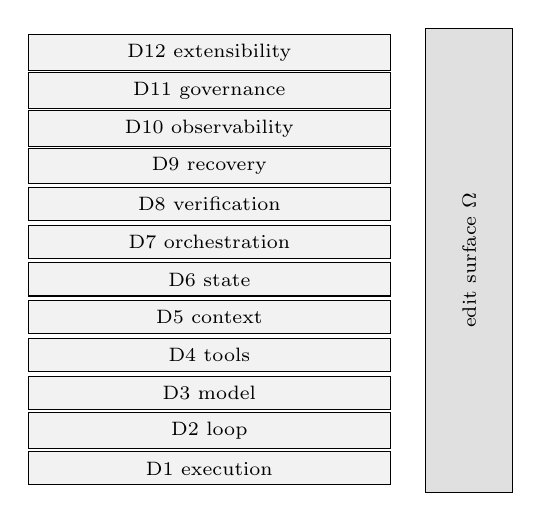
\begin{tikzpicture}[font=\scriptsize,node distance=1.6mm]
\foreach \i/\lab in {0/{D12 extensibility},1/{D11 governance},2/{D10 observability},3/{D9 recovery},4/{D8 verification},5/{D7 orchestration},6/{D6 state},7/{D5 context},8/{D4 tools},9/{D3 model},10/{D2 loop},11/{D1 execution}}{
  \node[draw,fill=black!5,minimum width=4.6cm,minimum height=0.42cm] (n\i) at (0,-\i*0.48) {\lab};
}
\node[draw,fill=black!12,minimum width=1.1cm,minimum height=5.9cm] at (3.3,-2.64) {};
\node[font=\scriptsize,rotate=90,align=center] at (3.3,-2.64) {edit surface $\Omega$};
\end{tikzpicture}
\caption{UHRM as a canonical partitioning of the harness edit surface. The model is the coarsest partition admitting sound, injective projections from all four source taxonomies.}
\label{fig:uhrm}
\end{figure}

\section{Self-Evolving Harnesses: A Comparative Protocol}
\label{sec:comparative}

Existing comparisons of harness-adaptation systems are made difficult by the absence of shared descriptors. We propose a ten-axis protocol: any system that modifies a harness must state (A1) the \emph{adaptation locus}, i.e.\ which UHRM dimensions are editable; (A2) the \emph{trigger}, i.e.\ when adaptation occurs relative to deployment; (A3) the \emph{evidence source}; (A4) \emph{label access}; (A5) the \emph{selection rule} that accepts or reverts a candidate; (A6) whether \emph{weights} are updated; (A7) the \emph{persistence} of the adapted artifact; (A8) the \emph{transfer protocol}; (A9) reported \emph{failure modes}; and (A10) reported \emph{safety and governance} metrics. Table~\ref{tab:comparative} applies the protocol to the four systems.

\begin{table*}[t]
\caption{Ten-axis comparison of self-evolving harness systems. All values are taken from the cited papers; ``n/r'' denotes not reported.}
\label{tab:comparative}
\centering
\footnotesize
\begin{tabular}{@{}p{2.5cm}p{3.4cm}p{3.4cm}p{3.4cm}p{3.4cm}@{}}
\toprule
\textbf{Axis} & \textbf{AHE}~\cite{b3} & \textbf{Self-Harness}~\cite{b4} & \textbf{TTHE}~\cite{b5} & \textbf{HarnessDev}~\cite{b6} \\
\midrule
A1 Locus & 7 editable component types exposed as files (prompt, tools, middleware, memory, \dots) & Declared harness interfaces (prompt, tools, runtime, verification) & Executable harness program: context construction, tool grounding, contract checks, recovery branches & Entire runnable harness codebase (multi-file) \\
A2 Trigger & Iterative offline rounds (10 iterations) & Iterative offline loop (3 stages) & \emph{Test time}, per unlabeled batch & Creation then Evolution; both pre-deployment \\
A3 Evidence & Layered, drill-down trajectory corpus distilled from millions of tokens & Clustered execution traces (weakness mining) & Unlabeled execution traces + execution-derived proxy signals & Downstream execution feedback (SWE-Pro-100, Terminal-Bench-89) \\
A4 Labels & Task-level outcomes, consulted after edit & Benchmark pass labels on held-in split & \emph{Label-free}; gold used only for measurement & Visible feedback set; 630-instance held-out split withheld \\
A5 Selection & Change manifest: keep if self-declared prediction verified next round; revert at file granularity & Accept only edits that pass regression testing & Agentic judge commits one candidate from proxy signals & Official version must complete both formal evaluations \\
A6 Weights & Frozen & Frozen & Frozen & Frozen \\
A7 Persistence & Persistent files & Persistent harness & Selected program governs subsequent inputs & Frozen, versioned, runnable harness \\
A8 Transfer & SWE-bench-Verified; 3 alternate model families (+5.1 to +10.1 pp) & Held-in and held-out splits, 3 benchmarks $\times$ 3 models & Transductive (same batch); cross-model check on BIRD & Held-out-630; fixed-executor (Gemini) transfer \\
A9 Failure modes & Components interact non-additively; self-attribution blind to regressions & n/r & Non-monotonic in search budget; judge selection regret; proxy unreliability & Unstable gains; partial transfer; executor-specific brittleness \\
A10 Safety & n/r & n/r & n/r & n/r \\
\bottomrule
\end{tabular}
\end{table*}

\subsection{Two Convergences and One Hard Divergence}

\textbf{Convergence 1: weights are frozen in all four systems.} This is what distinguishes harness engineering from fine-tuning or test-time training. It is also what makes the reported gains attributable to $H$ rather than to $M$, provided the harness condition is fully disclosed---the caveat that motivates Section~\ref{sec:hers}.

\textbf{Convergence 2: all four select on execution-derived evidence rather than on human judgement.} AHE verifies self-declared predictions against next-round outcomes, Self-Harness regression-tests, TTHE judges on proxy signals, and HarnessDev requires formal evaluation completion. Selection is therefore only as reliable as the evidence, which is the binding constraint the systems themselves identify.

\textbf{Divergence: label access partitions the field.} The four systems occupy three incompatible regimes. AHE and Self-Harness assume access to task-level labels during adaptation. HarnessDev assumes a visible feedback set drawn from the same distribution as the held-out split. TTHE assumes \emph{no} labels and adapts on the test batch itself. A gain reported under one regime carries no implication for another: a system that optimizes against labels can in principle be strictly more effective than a label-free system while telling us nothing about label-free adaptation, and vice versa. We return to the consequence in Section~\ref{sec:synthesis}.

\subsection{The Adaptation-Time Axis}

Fig.~\ref{fig:adapt} places the four systems on the two axes that most strongly determine comparability: when adaptation occurs and what supervision it consumes. HarnessDev's Creation stage is the only point that asks a model to build a harness from a weak seed; TTHE is the only point that adapts without labels. The lower-right region---test-time, label-free, held-out evaluation---is empty, and that emptiness is itself a finding: no system demonstrates label-free test-time adaptation measured on data it did not adapt to.

\begin{figure}[t]
\centering
\resizebox{\columnwidth}{!}{%
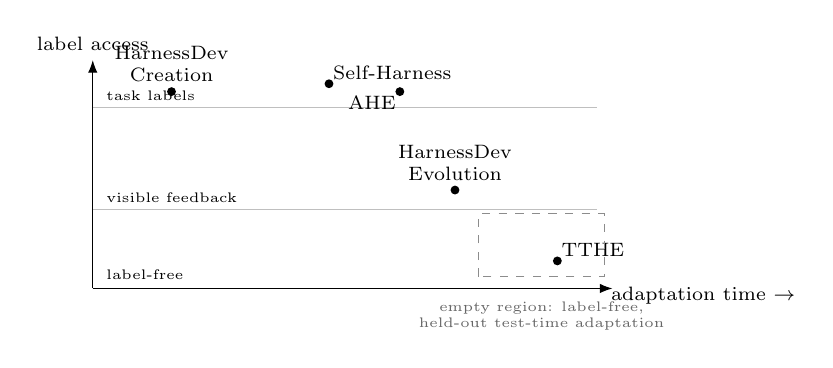
\begin{tikzpicture}[font=\scriptsize,scale=1.0]
\draw[-{Latex[length=1.6mm]}] (0,0) -- (6.6,0) node[below right=-2mm] {adaptation time $\rightarrow$};
\draw[-{Latex[length=1.6mm]}] (0,0) -- (0,2.9) node[above,align=center] {label access};
\node[anchor=west,font=\tiny] at (0.05,2.45) {task labels};
\node[anchor=west,font=\tiny] at (0.05,1.15) {visible feedback};
\node[anchor=west,font=\tiny] at (0.05,0.18) {label-free};
\draw[black!25] (0,2.3)--(6.4,2.3);
\draw[black!25] (0,1.0)--(6.4,1.0);
\fill (1.0,2.5) circle (1.6pt) node[above,align=center] {HarnessDev\\Creation};
\fill (3.0,2.6) circle (1.6pt) node[above right=-1mm,align=left] {Self-Harness};
\fill (3.9,2.5) circle (1.6pt) node[below left=-1mm,align=center] {AHE};
\fill (4.6,1.25) circle (1.6pt) node[above,align=center] {HarnessDev\\Evolution};
\fill (5.9,0.35) circle (1.6pt) node[above right=-1mm,align=center] {TTHE};
\draw[dashed,black!45] (4.9,0.15) rectangle (6.5,0.95);
\node[font=\tiny,align=center,black!60] at (5.7,-0.35) {empty region: label-free,\\held-out test-time adaptation};
\end{tikzpicture}}
\caption{The adaptation-time/supervision plane. The four systems occupy three mutually non-comparable regimes. The dashed region---label-free test-time adaptation evaluated on unseen data---is unoccupied.}
\label{fig:adapt}
\end{figure}

\section{Synthesis of Reported Gains}
\label{sec:synthesis}

\subsection{A Common Effect Scale}

Absolute point gains are not comparable across benchmarks with different headroom. We therefore re-express each reported gain on a ceiling-normalized scale. For an initial harness score $S_0$ and a final score $S_1$ on the same benchmark, model, and metric, we use
\begin{equation}
\gamma \;=\; \frac{S_1 - S_0}{100 - S_0},
\qquad
\rho \;=\; \frac{S_1 - S_0}{S_0},
\end{equation}
where $\gamma$ is the fraction of the remaining headroom to a perfect score that the harness recovers, and $\rho$ is the relative gain. Both are computed by us from published numbers; neither is reported by the source systems. Table~\ref{tab:gains} lists every reported harness gain we could normalize across the benchmarks used by the corpus: BIRD~\cite{b14}, LiveCodeBench~\cite{b15}, SWE-bench Verified~\cite{b10}, DS-1000~\cite{b13}, AppWorld~\cite{b12}, and Terminal-Bench~\cite{b11}.

\begin{table*}[t]
\caption{Reported harness gains re-expressed on a common scale. $S_0$ and $S_1$ are the initial and final harness scores exactly as published; $\Delta$, $\rho$, and $\gamma$ are recomputed by us. Metrics differ across rows (pass@1, official-verifier pass rate, graded score), so rows are comparable only within a benchmark.}
\label{tab:gains}
\centering
\footnotesize
\begin{tabular}{@{}llrrrrr@{}}
\toprule
\textbf{System} & \textbf{Benchmark} & \textbf{Model} & \textbf{$S_0 \to S_1$} & \textbf{$\Delta$} & \textbf{$\rho$} & \textbf{$\gamma$} \\
\midrule
AHE~\cite{b3}            & Terminal-Bench 2      & (frozen base)          & 69.7 $\to$ 77.0 & +7.3  & 0.105 & 0.241 \\
Self-Harness~\cite{b4}   & Terminal-Bench-2.0    & MiniMax M2.5           & 42.2 $\to$ 53.9 & +11.7 & 0.277 & 0.202 \\
Self-Harness~\cite{b4}   & Terminal-Bench-2.0    & Qwen3.5-35B-A3B        & 18.0 $\to$ 36.7 & +18.7 & 1.039 & 0.228 \\
Self-Harness~\cite{b4}   & Terminal-Bench-2.0    & GLM-5                  & 46.1 $\to$ 57.0 & +10.9 & 0.236 & 0.202 \\
Self-Harness~\cite{b4}   & SWE-bench Verified    & MiniMax M2.5           & 46.0 $\to$ 52.5 & +6.5  & 0.141 & 0.120 \\
Self-Harness~\cite{b4}   & SWE-bench Verified    & Qwen3.5-35B-A3B        & 19.5 $\to$ 41.5 & +22.0 & 1.128 & 0.273 \\
Self-Harness~\cite{b4}   & SWE-bench Verified    & GLM-5                  & 52.0 $\to$ 55.5 & +3.5  & 0.067 & 0.073 \\
Self-Harness~\cite{b4}   & AppWorld              & MiniMax M2.5           & 48.6 $\to$ 58.9 & +10.3 & 0.212 & 0.200 \\
Self-Harness~\cite{b4}   & AppWorld              & Qwen3.5-35B-A3B        & 22.5 $\to$ 52.2 & +29.7 & 1.320 & 0.383 \\
Self-Harness~\cite{b4}   & AppWorld              & GLM-5                  & 44.4 $\to$ 85.0 & +40.6 & 0.914 & 0.730 \\
TTHE~\cite{b5}           & BIRD (hard slice)     & DeepSeek V4 Flash      & 12.0 $\to$ 50.0 & +38.0 & 3.167 & 0.432 \\
TTHE~\cite{b5}           & LiveCodeBench         & DeepSeek V4 Flash      & 30.0 $\to$ 38.3 & +8.3  & 0.277 & 0.119 \\
TTHE~\cite{b5}           & SWE-bench Verified    & DeepSeek V4 Flash      & 20.0 $\to$ 35.0 & +15.0 & 0.750 & 0.188 \\
TTHE~\cite{b5}           & DS-1000               & DeepSeek V4 Flash      & 38.0 $\to$ 44.0 & +6.0  & 0.158 & 0.097 \\
TTHE~\cite{b5}           & claw-eval (graded)    & DeepSeek V4 Flash      & 48.9 $\to$ 69.8 & +20.9 & 0.427 & 0.409 \\
HarnessDev~\cite{b6}     & 5-benchmark mean (Creation) & Opus 4.8         & 0.0 $\to$ 67.8  & +67.8 & ---   & 0.678 \\
\bottomrule
\end{tabular}
\end{table*}

\subsection{The Apparent Ordering Is an Evaluation Artifact}

Read naively, Table~\ref{tab:gains} suggests that TTHE dominates: it reports the largest absolute gain and four of the highest $\rho$ values, without labels. Normalizing changes the picture. The mean ceiling-normalized gain is $\bar{\gamma}=0.268$ for Self-Harness (nine cells) and $\bar{\gamma}=0.249$ for TTHE (five cells, including the different-metric claw-eval row; excluding it, $0.209$), while AHE contributes a single datum at $\gamma=0.241$. These means lie well within one standard deviation of one another---the standard deviation of $\gamma$ within Self-Harness alone is $0.183$---and the spread \emph{within} Self-Harness (0.073 to 0.730) exceeds the spread \emph{between} the three systems (0.209 to 0.268). The apparent ordering is therefore not supported once headroom is accounted for.

Four confounds explain most of the residual differences.

\textbf{Confound 1: transductive evaluation.} TTHE scores each batch with the harness committed for that batch, so the adapted artifact is measured on the data it adapted to~\cite{b5}. The authors state this explicitly and its magnitude should not be compared to the held-out figures of other systems. Rows for AHE (cross-family transfer), Self-Harness (held-out splits), and HarnessDev (held-out-630) are of a different kind.

\textbf{Confound 2: slice conditioning.} TTHE's BIRD slice is constructed from 50 questions the baseline repeatedly failed~\cite{b5}. Its 12.0\% start is therefore low by construction, and its $+38.0$ gain measures recovery on known-hard queries rather than a general improvement. This row alone contributes the highest $\rho$ in the table ($3.167$) and would be misleading if quoted without the conditioning.

\textbf{Confound 3: visible feedback versus withheld data.} HarnessDev's Evolution feedback set is shown to the creator, and the authors report that gains shrink on held-out tasks: the largest held-out improvement is $+4.44$ points (Opus 4.8), and under a fixed Gemini executor only Opus improves on held-out data while other lineages regress~\cite{b6}. The Creation row in Table~\ref{tab:gains} is a different regime again---it measures construction from a zero-scoring seed, not evolution.

\textbf{Confound 4: ceiling and floor effects.} Normalization by $(100-S_0)$ is a convenience, not a model of achievable headroom. Where a human-engineered reference exists it is a better ceiling. HarnessDev reports human references of 80.0 on SWE-Pro and 88.8 on Terminal-Bench 2.1, with the best created harness at 67.8 on a five-benchmark mean against a human mean of 86.2~\cite{b6}; against the human ceiling, the gap is 18.4 points. A ceiling estimated from human performance would change $\gamma$ for every row in Table~\ref{tab:gains}, and no source system justifies its chosen denominator.

\subsection{Harness Sensitivity and Non-Additivity}

Two findings in the corpus constrain how much of a gain can ever be attributed to the harness. First, harness sensitivity can rival model replacement: the GPT-5 datum (35.2\% vs 49.6\% on Terminal-Bench 2.1 across two harnesses, weights fixed~\cite{b6}) exceeds the $+7.3$ point gain AHE obtains from ten evolution iterations. Harness choice and harness evolution are thus different levers, and the former is currently the larger one.

Second, harness components interact non-additively. AHE's ablation localizes its gain to tools, middleware, and long-term memory, while the system prompt \emph{alone} regresses performance~\cite{b3}; the authors conclude that stacking individually effective edits caps the aggregate gain. This is the evolution-loop analogue of the coupling problem identified at ecosystem scale in~\cite{b2}: local optimization of a coupled control system is fragile, and a component that looks beneficial in isolation can degrade the whole rollout.

\subsection{Efficiency Is Reported but Not Correlated with Quality}

Harness adaptation has a cost, and the reported evidence does not support ``more spend, better harness.'' AHE's frozen harness uses 12\% fewer tokens than its seed on SWE-bench-Verified while achieving the highest aggregate success~\cite{b3}. HarnessDev reports roughly nineteen-fold variation in MLE-bench token use across creators that does not reliably predict score; Gemini adds the fewest lines (1,006) yet obtains the best Terminal-Bench score (68.8), while the 18 code artifacts together add 17,111 net lines~\cite{b6}. Edit size and token spend are therefore poor proxies for harness quality, which strengthens the case for the reportable-budget field in HERS.

\section{A Reporting Standard for Harness Evolution}
\label{sec:hers}

The Harness Condition Sheet of~\cite{b7} requires that a benchmark run or deployment study record context artifacts, tool and protocol exposure, permission and network policy, execution substrate, persistence features, verification stack, recovery mechanisms, delegation topology, human approval rules, and cost or time budgets. This is necessary but insufficient for evolution studies, which must additionally disclose \emph{what was edited}, \emph{on what evidence}, and \emph{under what supervision}. Table~\ref{tab:hers} specifies the Harness Evolution Reporting Standard (HERS): the original condition fields, plus twelve evolution-specific fields drawn from the axes of Section~\ref{sec:comparative}.

\begin{table}[t]
\caption{The Harness Evolution Reporting Standard (HERS). Group A extends the Harness Condition Sheet of~\cite{b7}; Group B is new and required for any claim of harness improvement.}
\label{tab:hers}
\centering
\footnotesize
\begin{tabular}{@{}p{0.9cm}p{3.0cm}p{3.6cm}@{}}
\toprule
\textbf{ID} & \textbf{Field} & \textbf{Requirement} \\
\midrule
\multicolumn{3}{@{}l}{\textit{Group A --- Harness condition (after~\cite{b7})}} \\
A1 & Context artifacts & Files, memory, skills, retrieval sources \\
A2 & Tool/protocol exposure & Tool inventory; MCP/ACP/A2A~\cite{b21} surfaces \\
A3 & Permission \& network policy & Approval rules; allow/deny lists; egress \\
A4 & Execution substrate & Sandbox type; OS isolation; reset semantics \\
A5 & Persistence features & State store; checkpointing; resume/fork \\
A6 & Verification stack & Verifiers; synchronous vs.\ offline checks \\
A7 & Recovery mechanisms & Retry policy; rollback; failure taxonomy \\
A8 & Delegation topology & Sub-agents; roles; handoff protocol \\
A9 & Human approval rules & Gating points; intervention budget \\
A10 & Cost/time budget & Token, wall-clock, and step limits \\
\midrule
\multicolumn{3}{@{}l}{\textit{Group B --- Evolution disclosure (new)}} \\
B1 & Adaptation locus & UHRM dimensions edited (Table~\ref{tab:crosswalk}) \\
B2 & Adaptation trigger & Creation / offline rounds / test time \\
B3 & Editable surface size & Files, LOC, parameters exposed \\
B4 & Evidence source & Traces, feedback, proxy signals \\
B5 & Label access & None / held-in / visible feedback \\
B6 & Selection rule & Acceptance and revert semantics \\
B7 & Rollback semantics & Granularity of reversion \\
B8 & Weight-update status & Frozen or updated (with justification) \\
B9 & Artifact persistence & Versioning; reproducibility of the artifact \\
B10 & Transfer protocol & Held-out splits; cross-model; cross-executor \\
B11 & Adaptation budget & Iterations, rollouts, proposer tokens \\
B12 & Safety \& governance metrics & Unsafe-action rate; approval burden \\
\bottomrule
\end{tabular}
\end{table}

\section{Open Problems and Research Agenda}
\label{sec:open}

\textbf{1) Governance of self-modifying harnesses.} The most uniform omission in the corpus is also the most consequential. Table~\ref{tab:comparative}, axis A10, is ``not reported'' for every system: none of AHE, Self-Harness, TTHE, or HarnessDev reports an unsafe-action rate, a permission-boundary violation, or a human-intervention burden for its self-modified harness. This is not a criticism of individual papers---none set out to measure governance---but it is a structural gap. A system that edits the layer through which an agent obtains authority is exactly the system for which the authority delta must be measured. The Control Plane framework already formalizes the required quantities (unsafe action rate, human intervention burden)~\cite{b7}; what is missing is their application to evolved harnesses. A minimal first study would report the UHRM dimensions touched by each accepted edit, the permission-relevant surface exposed after adaptation, and the change in unsafe-action rate relative to the seed under a fixed adversary model. The survey's call for unified adversarial benchmarks for governance stacks~\cite{b2} supplies the adversary model.

\textbf{2) Selection under unreliable proxies.} TTHE identifies execution-derived proxy reliability as a central challenge and quantifies it: a pool oracle shows roughly fourteen points already generated but left uncommitted, i.e.\ selection regret rather than generation failure~\cite{b5}. Reported harness performance is non-monotonic in search budget, with more rounds helping only when more proposers are used. The open question is precise: given a fixed budget and a proxy whose fidelity is unknown, what selection rule maximizes held-out gain? This is a bandit problem with a biased reward signal, and none of the four systems states its proxy's calibration.

\textbf{3) Regression foresight.} AHE reports that its loop's self-attribution is reliable for fixes but blind to regressions~\cite{b3}; HarnessDev reports that evolution gains are unstable and transfer only partially, with lineages regressing under a fixed executor~\cite{b6}. Both point to the same missing capability: predicting, before committing an edit, which previously passing behaviours it will break. Self-Harness's regression-testing acceptance rule~\cite{b4} is the only mechanism in the corpus aimed at this, and it is a filter rather than a predictor. A predictor would need per-edit impact attribution, which HERS field B1 is designed to make possible.

\textbf{4) Comparability by construction.} The confounds of Section~\ref{sec:synthesis} are not incidental. No benchmark in the corpus varies the harness while holding the model, data, and evaluation protocol fixed across multiple evolution methods. Terminal-Bench 2 is used by AHE and Self-Harness under different base models and different harnesses; HarnessDev's contribution is precisely to make the harness the unit of evaluation, but it evaluates creators, not evolution algorithms head-to-head. A \emph{harness-ablation benchmark}---fixed model, fixed task distribution, multiple adaptation algorithms, held-out evaluation, mandated HERS reporting---would let the field answer whether any evolution method dominates another.

\textbf{5) Recovery and state persistence.} HarnessDev finds that while 11 of 18 created code harnesses define a state class, only one exposes a state-saving interface and only one implements periodic checkpointing; no checkpoint event appears across 26{,}679 recorded task trajectories~\cite{b6}. Recovery is the least-implemented UHRM dimension relative to its importance for long-horizon tasks, and it is precisely the dimension that the Control Plane frames as a first-class outcome alongside one-shot success~\cite{b7}. Whether recoverability is better predicted by loop design (D2) or by state persistence (D6) is an open empirical question.

\textbf{6) Termination and saturation.} AHE's ten iterations and the non-monotonic budget curves of TTHE both imply that evolution has a stopping problem: gains are not monotone in effort, and the systems do not state a principled stopping criterion. As base models improve, the harness headroom shrinks for reasons unrelated to harness quality---which motivates the survey's open question of how to \emph{simplify} harnesses as models improve~\cite{b2}. A saturation-aware objective would treat harness complexity as a cost, not only token spend.

\section{Threats to Validity}
\label{sec:threats}

\textit{Secondary analysis.} Every number in Table~\ref{tab:gains} is recomputed from a published figure; we ran no experiment. Where a source reports a distribution (e.g.\ avg@3 over three independent harnesses in~\cite{b6}) we used its reported mean, so our $\gamma$ inherits the source's variance, which we do not propagate. \textit{Heterogeneous metrics.} Rows of Table~\ref{tab:gains} span pass@1, official-verifier pass rates, and a graded score in $[0,1]$; normalization by a 100-point ceiling is a convenience that assumes a comparable scale, and the claw-eval row is explicitly not comparable to the others. \textit{Taxonomy construction.} The UHRM depends on the semantic alignment encoded in the projections $\pi_i$; a reader who disputes an alignment would obtain a different crosswalk. We mitigate this by stating the soundness, injectivity, and coarseness conditions explicitly so that any disputed cell can be revised without changing the construction. \textit{Preprint status.} All sources are 2026 preprints or technical reports; several may be revised, and the quantitative claims of Section~\ref{sec:synthesis} track the versions cited. \textit{Selection of systems.} We compare the four self-evolving systems known to us at the time of writing; the corpus is young and the comparison is not claimed to be exhaustive.

\section{Conclusion}

An LLM agent is a model plus a harness, and the harness has become a first-class engineering surface: with weights frozen, harness choice alone moves Terminal-Bench 2.1 success by 14.4 points. This paper argued that the field's rapid growth has outrun its vocabulary. We formalized compatibility between harness taxonomies via sound, injective projections, and derived the 12-dimensional UHRM, whose crosswalk shows that each of the four leading taxonomies omits concerns the others name---model integration, observability, recovery, extensibility. We defined a ten-axis protocol for harness-adaptation systems and found that all four self-evolving systems freeze weights, all select on execution-derived evidence, and all diverge on the single axis that most determines comparability: label access. Re-normalizing every reported gain onto a common headroom scale dissolved the apparent ranking between systems, and the residual differences were attributable to four confounds---transductive evaluation, slice conditioning, visible feedback, and unspecified ceilings---that we proposed HERS to control. The sharpest finding is a uniform omission: no self-evolution system reports a safety or governance metric for the harness it modified. Measuring the authority delta of a self-modified harness is, in our view, the most urgent open problem in the field.

\begin{thebibliography}{00}

\bibitem{b1} P. Barbaste, T. Darrigol, G. Vu, and T. Wiltberger, ``Harness engineering: Anatomy, architecture, and evolution of coding agents --- a source-code study of eleven systems,'' arXiv:2609.00006, Jul. 2026.

\bibitem{b2} J. Li, X. Xiao, Y. Zhang, C. Liu, L. Zhao, et al., ``Agent harness engineering: A survey,'' 2026. [Online]. Available: https://picrew.github.io/LLM-Harness/

\bibitem{b3} J. Lin, S. Liu, C. Pan, L. Lin, S. Dou, Z. Xi, X. Huang, H. Yan, Z. Han, T. Gui, and Y.-G. Jiang, ``Agentic harness engineering: Observability-driven automatic evolution of coding-agent harnesses,'' arXiv:2604.25850, May 2026.

\bibitem{b4} H. Zhang, S. Zhang, K. Li, C. Zhang, Y. Chen, Y. Zhang, L. Bai, and S. Hu, ``Self-Harness: Harnesses that improve themselves,'' arXiv:2606.09498, Aug. 2026.

\bibitem{b5} J. Nie, Y. Zhang, J. Song, Q. Cai, D. Yu, Y. Guo, X. Tian, and B. Han, ``TTHE: Test-time harness evolution,'' arXiv:2607.08124, Jul. 2026.

\bibitem{b6} ByteDance Seed et al., ``HarnessDev: Can LLMs create and evolve their own agent harness?'' arXiv:2609.01437, Sep. 2026.

\bibitem{b7} C. Mishra, ``Harness-native software engineering: The control plane of coding agents,'' Mar. 2026. [Online]. Available: https://research.chaitanya.science/

\bibitem{b8} J. Kim, ``Harness engineering: A governance framework for AI-driven software engineering,'' Zenodo, Mar. 2026, doi: 10.2139/ssrn.6372119.

\bibitem{b9} S. Yao, J. Zhao, D. Yu, N. Du, I. Shafran, K. Narasimhan, and Y. Cao, ``ReAct: Synergizing reasoning and acting in language models,'' in \emph{Proc. ICLR}, 2023.

\bibitem{b10} C. E. Jimenez, J. Yang, A. Wettig, S. Yao, K. Pei, O. Press, and K. Narasimhan, ``SWE-bench: Can language models resolve real-world GitHub issues?'' in \emph{Proc. ICLR}, 2024.

\bibitem{b11} The Terminal-Bench Team, ``Terminal-Bench: A benchmark for AI agents in terminal environments,'' Laude Institute, 2026. [Online]. Available: https://www.tbench.ai/

\bibitem{b12} H. Trivedi, T. Khot, M. Hartmann, R. Manku, V. Dong, E. Li, S. Gupta, A. Sabharwal, and N. Balasubramanian, ``AppWorld: A controllable world of apps and people for benchmarking interactive coding agents,'' in \emph{Proc. ACL}, 2024.

\bibitem{b13} Y. Lai, C. Li, Y. Wang, T. Zhang, R. Zhong, L. Zettlemoyer, S. W. Yih, D. Fried, S. Wang, and T. Yu, ``DS-1000: A natural and reliable benchmark for data science code generation,'' in \emph{Proc. ICML}, 2023.

\bibitem{b14} J. Li, B. Hui, G. Qu, J. Yang, B. Li, B. Li, B. Wang, B. Qin, R. Geng, N. Huo, et al., ``Can LLM already serve as a database interface? A big bench for large-scale database grounded text-to-SQLs,'' in \emph{Proc. NeurIPS}, 2023.

\bibitem{b15} N. Jain, K. Han, A. Gu, W.-D. Li, F. Yan, T. Zhang, S. Wang, A. Solar-Lezama, K. Sen, and I. Stoica, ``LiveCodeBench: Holistic and contamination-free evaluation of large language models for code,'' in \emph{Proc. ICLR}, 2025.

\bibitem{b16} N. Shinn, F. Cassano, E. Berman, A. Gopinath, K. Narasimhan, and S. Yao, ``Reflexion: Language agents with verbal reinforcement learning,'' in \emph{Proc. NeurIPS}, 2023.

\bibitem{b17} O. Khattab, A. Singhvi, P. Maheshwari, Z. Zhang, K. Santhanam, S. Vardhamanan, S. Haq, A. Sharma, T. T. Joshi, H. Moazam, et al., ``DSPy: Compiling declarative language model calls into self-improving pipelines,'' in \emph{Proc. ICLR}, 2024.

\bibitem{b18} B. Rombaut, ``Inside the scaffold: A source-code taxonomy of coding agent architectures,'' arXiv preprint, 2026.

\bibitem{b19} OpenAI, ``Harness engineering: Leveraging Codex in an agent-first world,'' 2026. [Online]. Available: https://openai.com/index/harness-engineering/

\bibitem{b20} Anthropic, ``Harness design for long-running application development,'' 2026. [Online]. Available: https://www.anthropic.com/engineering/harness-design-long-running-apps

\bibitem{b21} Anthropic, ``Model Context Protocol,'' 2024. [Online]. Available: https://modelcontextprotocol.io/

\end{thebibliography}

\end{document}
